\chapter{Sonar Simulation}

\epigraph{If you cause your ship to stop, and place the head of a long tube in
the water and place the outer extremity\\ in your ear, you will hear ships at a
great distance from you.}{\textit{Leonardo Da Vinci}, 1490}


The idea behind simulation is to have a flexible environment where the system
(e.g. sonar, reconstruction model) can be tested on a variety of conditions
and the ground truth is well known. It is a mature and widespread
mechanism for development of new sonar technologies \cite{Etter2013}.

Opening this chapter, it will be presented physical foundations behind sonars,
and its existing technologies and models. Next describing the envisioned
environmental properties, and ending  with  a more detailed view of the
simulation technique used.

\section{Sonar}

Throughout this thesis only one type of sonar is considered, the mechanical
imaging active sonar. Sonars have a comum underlying principle of operation, but
vary greatly on aplication and hardware constituition.

Sonars are, in some sense, the acoustic analog of a camera. They use sound,
instead of light, to capture information about the environment. So, to better
undersand \textit{how} they operate and \textit{what} are they used for, it is
important to have a clear concept of sound.

\subsection{Physics of Sound}

The phenomenon that humans percieve as sound is a pressure wave that amplitude
excess the mean pressure of the medium \cite{FEYNMAN}. It can me referred to as
\textit{compressional} or \textit{longitudinal} waves, contrasting with
\textit{transversal waves}. The difference between these two kinds of waves
relies on the direction of the movement of the particles, being parallel or
perpendicular to the propagation of the wave, respectively\cite{BRUNEAU}.

On the particular, but usefull, conditions of low energy
phenomena\cite{Lefebvre} (with some other suitable requirements\footnote{A
perfect simple fluid in an initial state of stationary homogeneous equilibrium})
the pressure pertubation wave can be described as the \textit{D'Alembert
equation}:
 
\begin{equation}\label{eq:lambert}
\nabla^2 \Phi - \frac{1}{c^2_0}\frac{\partial^2}{\partial t^2} \Phi = 0
\end{equation}

Where $\Phi$ is the velocity potencial, a scalar field that helps describing the
sound propagation. Its relation to sound pressure is:

\[ p =  -\rho \frac{\partial}{\partial t}\Phi \]

Which can be directly described as:

\begin{equation} \label{eq:wave}
\nabla^2 p - \frac{1}{c^2_0}\frac{\partial^2}{\partial t^2} p = 0
\end{equation} 
 
Where $p$ is the pressure deviation from the mediums, $\rho$ the density, $c_0$
is the local sound speed and $\nabla^2$ stands for the Laplace operator. These equations are
only valid in free space (no source), but discrete variations of the medium are
treated as boundary conditions, giving origin to reflection and refraction.

Besides pressure, sound has another important derived property: intensity. Much
like the case of electromagnetic waves, sound intensity (or acoustic intensity)
measures the mean value of the sound energy flux (i.e. energy rate
per area):

\begin{equation}\label{eq:intensity_mean}
\vec{I} = \overline{p\vec{v}}
\end{equation}

Where $\vec{I}$ represents the \textit{acoustic intensity} vector, $\vec{v}$ the
\textit{acoustic velocity} (i.e. the velocity of a particle in the medium) and the
overline the mean over some time period. The \textit{acoustic velocity} can also
be derived from the velocity potencial $\Phi$ as:

\[ \vec{v} = \nabla \Phi\]

When considering a wave far from its source, solutions to the equation
\ref{eq:wave} give rise to a \textit{plane wave}( where the coherent wave front
propagate in a plane). It makes clear the relationship between $\vec{v}$ and
$p$:

\[ \vec{v} = \frac{p}{\rho c_0} \vec{n_0} \]

Where $\vec{n_0}$ is the unit normal vector to the wavefront. Pluging it back to
equation \ref{eq:intensity_mean}:

\begin{equation}\label{eq:intensity_pressure}
\vec{I} = \tfrac{1}{\rho c_0} \overline{p^2} \vec{n_0}
\end{equation}

This equation shows the proportionality between the \textit{acoustic
intensity} and the mean squared of the pressure. The inverse of the
proportionality constant $\rho c_0$ is called the \textit{characteristic
impendace} because it measures the degree of ``resistense to propagation'' of
the medium.

%By means of the same reasoning about the physical properties

 %(perpendicular to the direction of propagation)

Because the acoustic intensity (and related quantities) varies orders of
magnitude while propagating, it is commom to quantify it on a logarithmic scale,
specifically \textit{decibels} (dB)\cite{LURTON}:

\begin{equation}\label{eq:dB}
I_{dB} = 10~\log_{10}\left(\frac{I}{I_0}\right)
\end{equation} 

Here $I_{dB}$ is the intensity measured in \textit{decibels}, $I$ the intensity
value and $I_0$ a reference intensity values, usually defined somewhere near the
source. In the case of reflected/refracted wave, $I_0$ may also refere to
the intensity of the incoming wave.

\subsection{Sonar Principle of Operation}

\cite{LURTON} % porra toda - principio de funcionamento

\subsection{Available Models}
 
\cite{sonars:16} % tipos de sonar

\section{Simulation}

Works on \textit{computacional ocean
acoustics}, the subfield of knowledge that explores the algorithms that model
the ocean as an acoustic medium, are well documented by
\citet{Etter2013}.

When constructing a simulation one has to consider the tradeoff between
simplicity/perfomance/accuracy.

\subsection{Techniques Overview}
\subsection{Ray Theory}
\subsection{3D Enviroment Specifics}
\subsection{Results}

\section{Environment}

\subsection{Modeling}
\subsection{Characterization}
\section{Implementation}
\subsection{Algorithm}

The implemented algorithm receives as input a sequence of sonar positions
$\mathbf{P}_k$ and its respective sonar responses, that is a sequence of beams
$\mathbf{b}_j^{(k)}$ containing bearing and bins values. The procedure goes
as illustrated in Algorithm \ref{alg:mapping}.


\begin{algorithm}
\caption{Mapping}
\label{alg:mapping}
\begin{algorithmic}
\Procedure{Mapping}{$\mathbf{P}_k,\mathbf{b}_j^{(k)}$}

\State $I_k = \{\mathbf{b}_j^{(k)}|j\in \mu\mathbb{N}\}$
\Comment{Partitioning at every $\mu$ beam}

\State $\coord{w}_0 = \mathbf{0}$
\ForAll{$\mathbf{P}_k$}
\ForAll{$\mathbf{b}\in I_k$}
\State $\mathbf{b} = \mathrm{threshold}(\mathbf{b})$
\Comment{Classify empty/full, section \ref{s:ism}}
\State $e_i = \mathrm{empty\_samples}(\mathbf{b})$
\Comment{Sample first empty bins, section \ref{ss:isfm}}
\State $f_i^{(z)} = \mathrm{full\_samples}(\mathbf{b})$
\Comment{Sample from every $z$ full bin, section \ref{ss:isfm}}
\State $\text{feats}=\{\}$

\ForAll{$e_i$}
\State $\text{feats}=\text{feats}\cup\{\hat\varphi(e_i)\}$
\Comment{equation \ref{eq:nystrom}}
\EndFor

\ForAll{$f^{(z)}$}
\State
$\text{feats}=\text{feats}\cup\{\mathbb{E}_i[{
\hat\varphi(f_i^{(z)})}]\}$
\Comment{equation \ref{eq:embedding}}
\EndFor
\EndFor

\State $\coord{w} {-=}
\eta_k\nabla\text{NLL}_{\text{reg}}(\coord{w}_t;\text{feats})$ 
\Comment{equation \ref{eq:leariningrate} on a variant of
\ref{eq:minibatch}}
\EndFor
\State \textbf{return} $\coord{w}$
\EndProcedure
\end{algorithmic}
\end{algorithm}

In the description of the algorithm
$\nabla\text{NLL}_{\text{reg}}(\coord{w}_t;\text{feats})$ has a slightly
different meaning:

\begin{equation*}
\nabla\text{NLL}_{\text{reg}}(\coord{w}_t;\text{feats}) =
\sum_{\hat{\mathbf{\varphi}}\in \text{feats}}
-y_t\hat{\mathbf{\varphi}}(1+\exp(y_i~ \coord{w}\cdot\hat{\mathbf{\varphi}})^{-1} +\lambda\nabla\mathcal{S}(\coord{w})
\end{equation*}


\subsection{Results}

Although the algorithm generates a 3D representation of an environment, results
displayed here are plane cuts of this reconstruction only for better
appreciation. The environment considered here is the 4x5 semi-inifinity box of
section \ref{eq:boxlikenv}. There were used $3000$ inducing points (dimension of
the feature map approximation - section \ref{sss:hilbertcontinuousmap}) and $21$
measurements from $7$ different positions in $3$ ortogonal orientations each
from the sonar simulation. Different fractions of the number of beams were
explored on figures \ref{fig:ten_map}, \ref{fig:thir_map} and
\ref{fig:full_map}. Colors represent the value of the occupancy
$p(x;\coord{w})$.

\begin{figure}[ht]
    \centering
    \subfloat[Plane
    $x=-1$]{{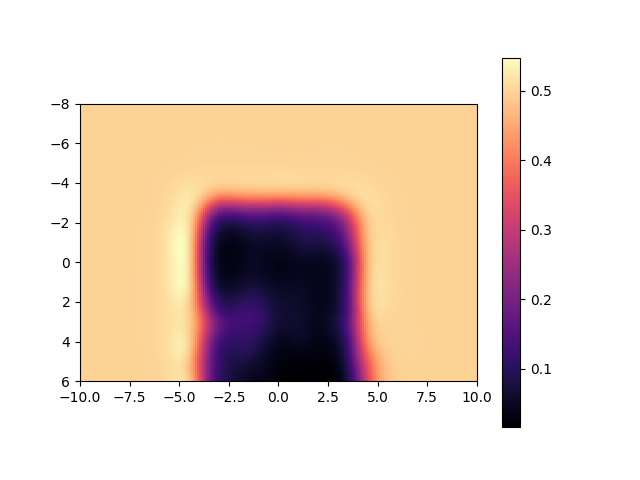
\includegraphics[width=75mm,trim={0 14mm 0
    10mm},clip]{Chap4/fig/ten_x_-1}}}%
    \hfill \subfloat[Plane
    $z=-2$]{{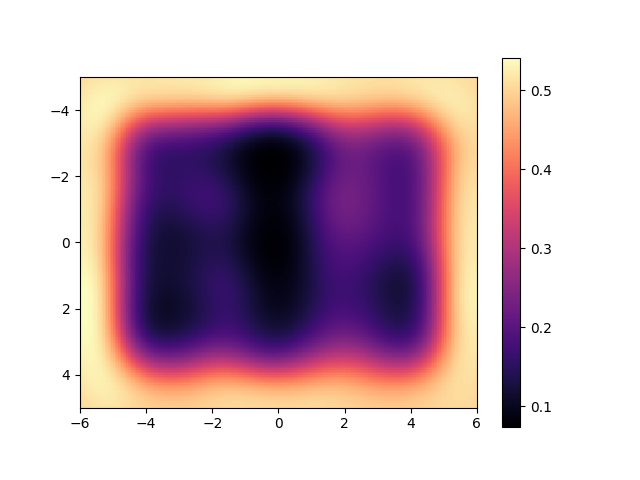
\includegraphics[width=75mm,trim={0 14mm 0
    10mm},clip]{Chap4/fig/ten_z_-2}}}%
    \\%
    \subfloat[Plane
    $x=0$]{{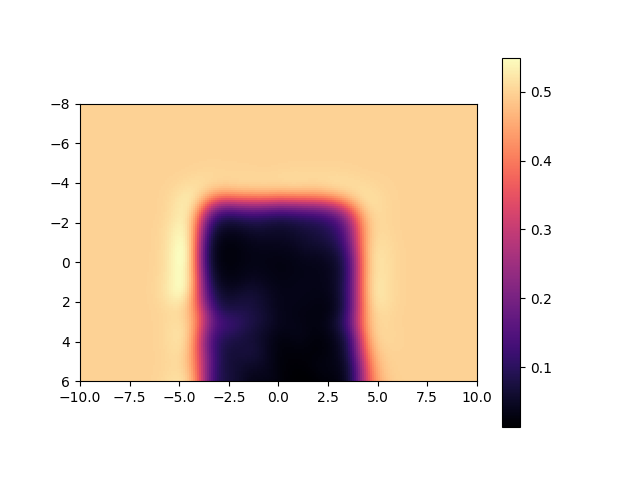
\includegraphics[width=75mm,trim={0 14mm 0
    10mm},clip]{Chap4/fig/ten_x_0}}}%
    \hfill \subfloat[Plane
    $z=-1$]{{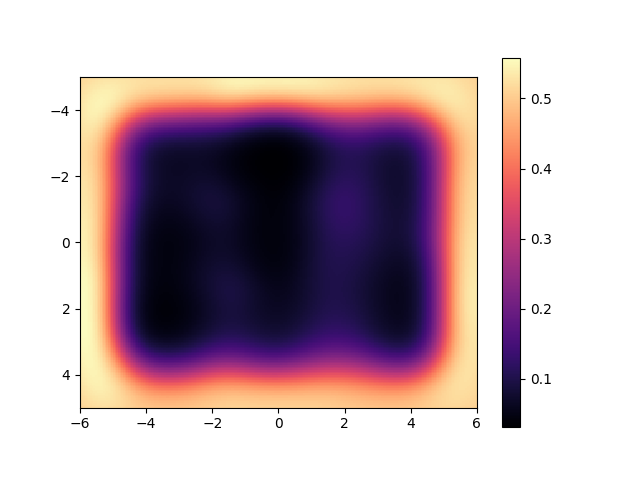
\includegraphics[width=75mm,trim={0 14mm 0
    10mm},clip]{Chap4/fig/ten_z_-1}}}%
    \\%
    \subfloat[Plane
    $x=1$]{{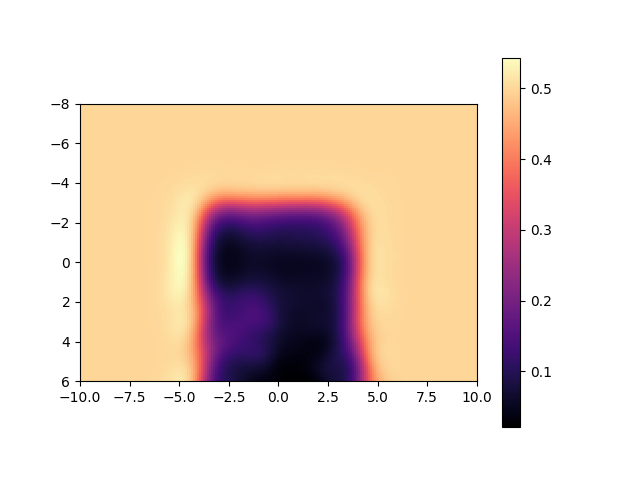
\includegraphics[width=75mm,trim={0 14mm 0
    10mm},clip]{Chap4/fig/ten_x_1}}}%
    \hfill \subfloat[Plane
    $z=0$]{{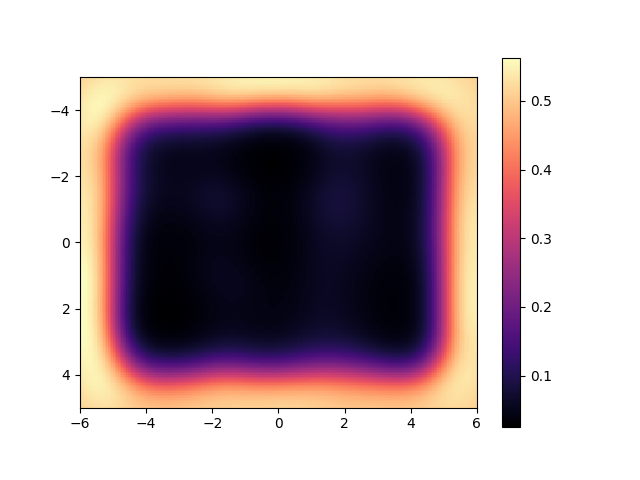
\includegraphics[width=75mm,trim={0 14mm 0
    10mm},clip]{Chap4/fig/ten_z_0}}}%
    \caption{Mapping with $10\%$ of available beams.}%
    \label{fig:ten_map}%
\end{figure}

\begin{figure}[ht]
    \centering
    \subfloat[Plane
    $x=-1$]{{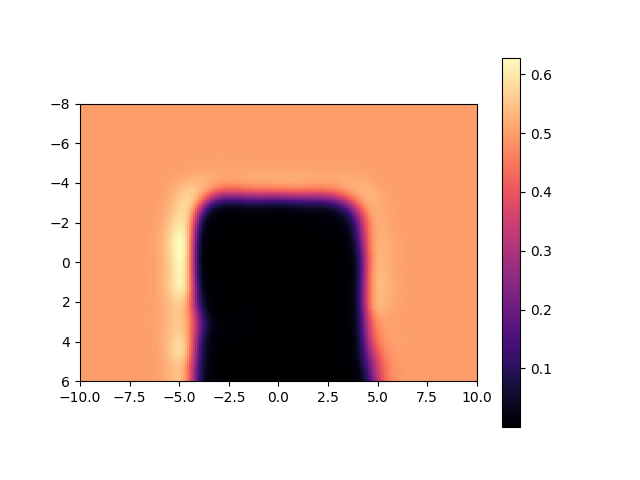
\includegraphics[width=75mm,trim={0 14mm 0
    10mm},clip]{Chap4/fig/thir_x_-1}}}%
    \hfill \subfloat[Plane
    $z=-2$]{{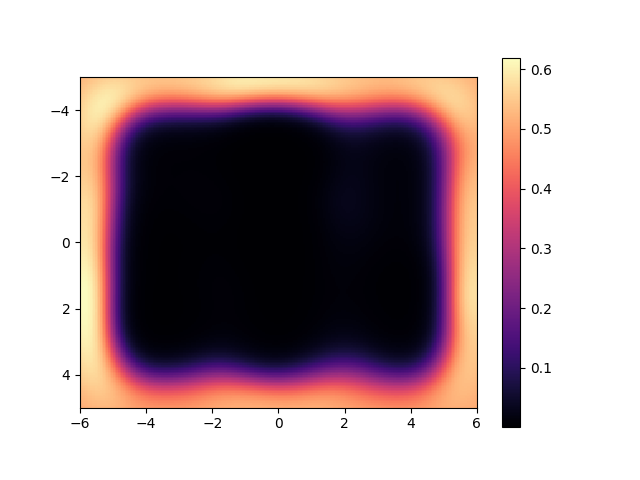
\includegraphics[width=75mm,trim={0 14mm 0
    10mm},clip]{Chap4/fig/thir_z_-2}}}%
    \\%
    \subfloat[Plane
    $x=0$]{{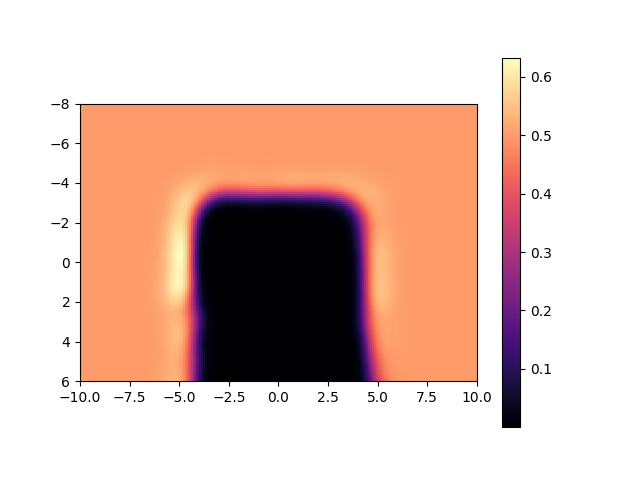
\includegraphics[width=75mm,trim={0 14mm 0
    10mm},clip]{Chap4/fig/thir_x_0}}}%
    \hfill \subfloat[Plane
    $z=-1$]{{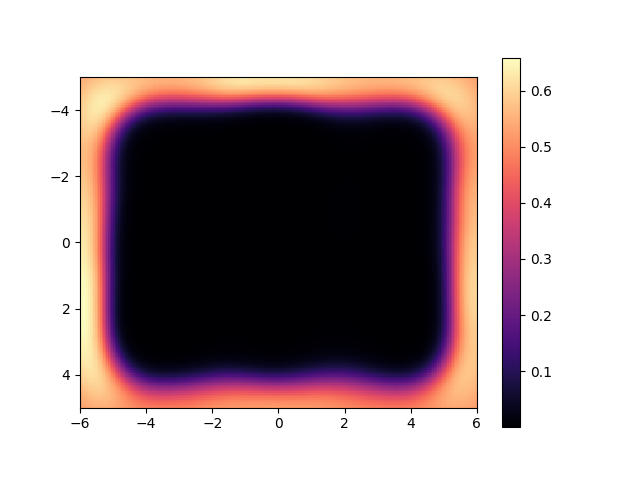
\includegraphics[width=75mm,trim={0 14mm 0
    10mm},clip]{Chap4/fig/thir_z_-1}}}%
    \\%
    \subfloat[Plane
    $x=1$]{{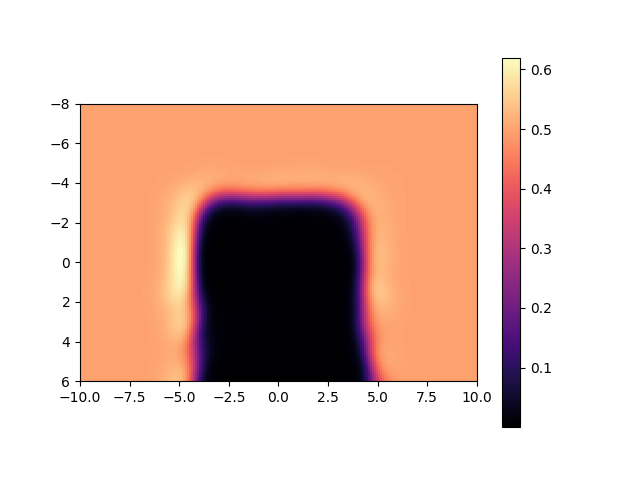
\includegraphics[width=75mm,trim={0 14mm 0
    10mm},clip]{Chap4/fig/thir_x_1}}}%
    \hfill \subfloat[Plane
    $z=0$]{{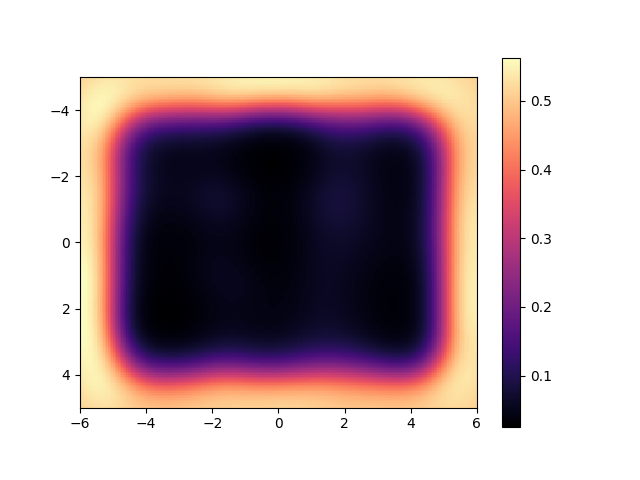
\includegraphics[width=75mm,trim={0 14mm 0
    10mm},clip]{Chap4/fig/ten_z_0}}}%
    \caption{Mapping with $30\%$ of available beams.}%
    \label{fig:thir_map}%
\end{figure}

\begin{figure}[ht]
    \centering
    \subfloat[Plane
    $x=-1$]{{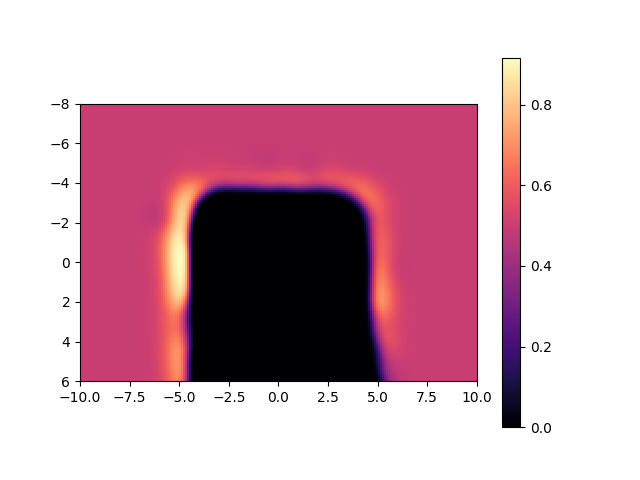
\includegraphics[width=75mm,trim={0 14mm 0
    10mm},clip]{Chap4/fig/full_x_-1}}}%
    \hfill \subfloat[Plane
    $z=-2$]{{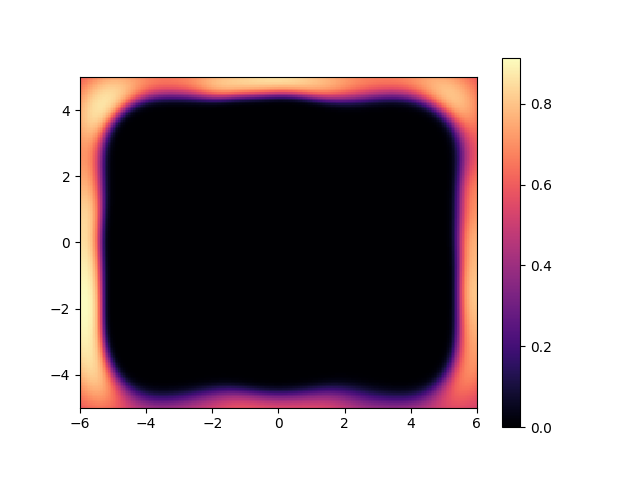
\includegraphics[width=75mm,trim={0 14mm 0
    10mm},clip]{Chap4/fig/full_z_-2}}}%
    \\%
    \subfloat[Plane
    $x=0$]{{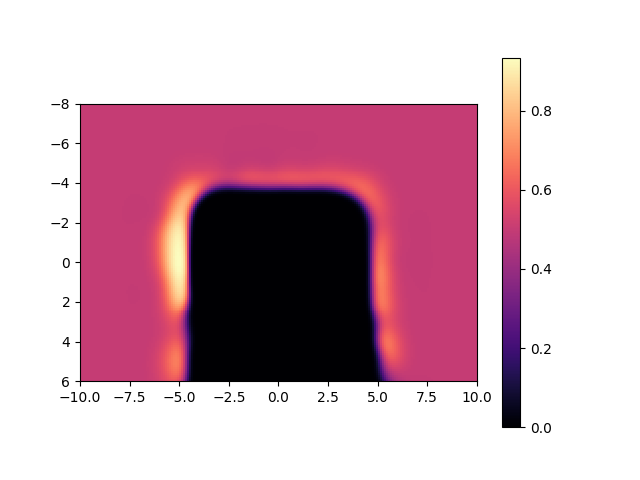
\includegraphics[width=75mm,trim={0 14mm 0
    10mm},clip]{Chap4/fig/full_x_0}}}%
    \hfill \subfloat[Plane
    $z=-1$]{{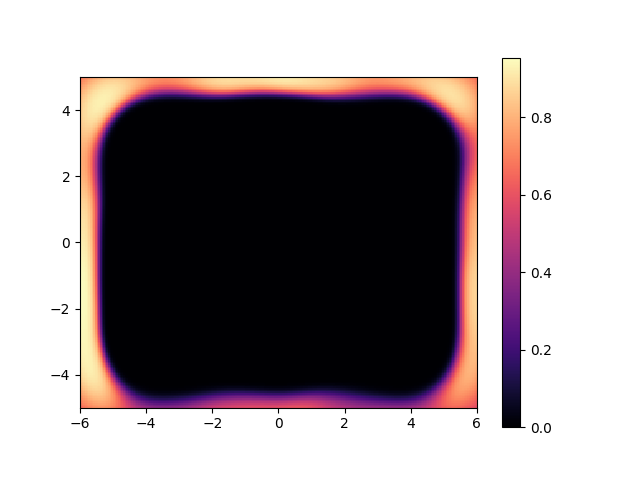
\includegraphics[width=75mm,trim={0 14mm 0
    10mm},clip]{Chap4/fig/full_z_-1}}}%
    \\%
    \subfloat[Plane
    $x=1$]{{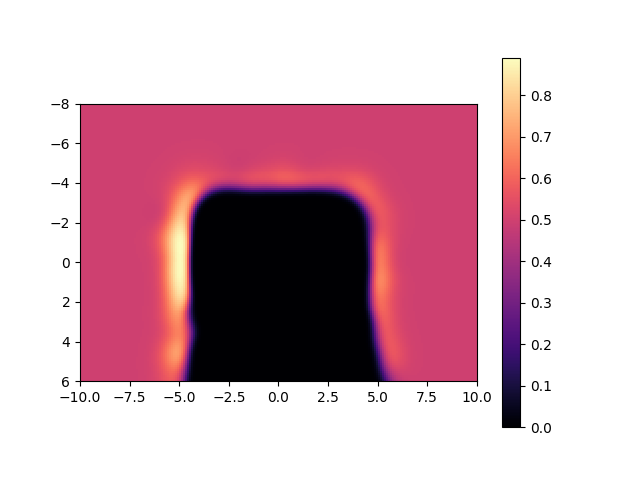
\includegraphics[width=75mm,trim={0 14mm 0
    10mm},clip]{Chap4/fig/full_x_1}}}%
    \hfill \subfloat[Plane
    $z=0$]{{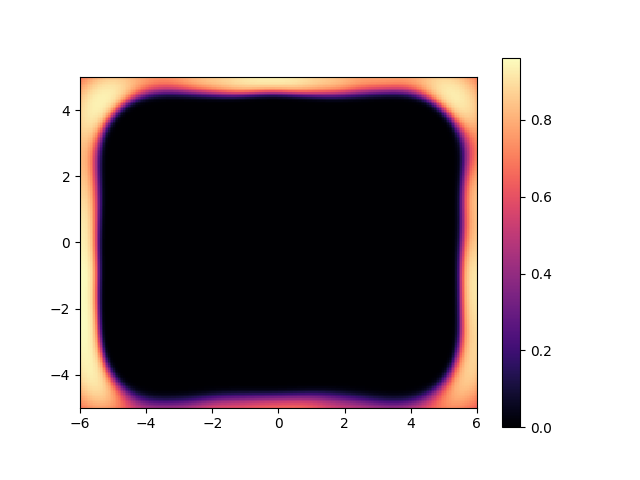
\includegraphics[width=75mm,trim={0 14mm 0
    10mm},clip]{Chap4/fig/full_z_0}}}%
    \caption{Mapping with $100\%$ of available beams.}%
    \label{fig:full_map}%
\end{figure}

